\documentclass[12pt,a4paper]{report}
\usepackage[utf8]{inputenc}
\usepackage[T1]{fontenc}
\usepackage{geometry}
\usepackage{graphicx}
\usepackage{xcolor}
\usepackage{titlesec}
\usepackage{fancyhdr}
\usepackage{hyperref}
\usepackage{array}
\usepackage{booktabs}
\usepackage{longtable}
\usepackage{enumitem}
\usepackage{listings}
\usepackage{tcolorbox}
\usepackage{mdframed}
\usepackage{tikz}
\usepackage{pgfplots}
\usepackage{float}
\usepackage{caption}
\usepackage{amsmath}
\usepackage{amssymb}
\usepackage{pifont}
\usepackage{setspace}
%\usepackage{microtype}
\usepackage{tabularx}
\usepackage{colortbl}
\usepackage{makecell}
\usepackage{parskip}
\usepackage{etoolbox}
\usepackage{afterpage}
\pgfplotsset{compat=1.18}
\usetikzlibrary{shapes.geometric,arrows.meta,positioning,backgrounds,fit}
\frenchspacing
\geometry{top=2.5cm,bottom=2.5cm,left=3cm,right=2.5cm,headheight=15pt}
\definecolor{primaryPurple}{HTML}{673AB7}
\definecolor{lightPurple}{HTML}{B19CD9}
\definecolor{accentPurple}{HTML}{9370DB}
\definecolor{cafeeGold}{HTML}{C9A84C}
\definecolor{cafeeNavy}{HTML}{1B2A4A}
\definecolor{cafeeCream}{HTML}{F5F0E8}
\definecolor{lightGray}{HTML}{F8F8F8}
\definecolor{darkGray}{HTML}{555555}
\definecolor{successGreen}{HTML}{2E7D32}
\definecolor{borderGray}{HTML}{DDDDDD}
\definecolor{accentTeal}{HTML}{00897B}
\hypersetup{colorlinks=true,linkcolor=primaryPurple,urlcolor=accentTeal,citecolor=cafeeNavy,pdftitle={Rapport de Stage - Soeurise},pdfauthor={Cafee Agency}}
\titleformat{\chapter}[display]
{\normalfont\bfseries\color{cafeeNavy}}
{\hfill\tikz[baseline=-0.6ex]{\fill[primaryPurple](0,0)rectangle(1.1cm,1.1cm);\node[white,font=\Large\bfseries]at(0.55cm,0.55cm){\thechapter};}}
{-4pt}{\Huge\raggedright}
[\vspace{4pt}{\color{primaryPurple}\hrule height 2pt}\vspace{6pt}]
\titleformat{\section}{\normalfont\Large\bfseries\color{cafeeNavy}}{\color{primaryPurple}\thesection}{0.8em}{}[\vspace{2pt}{\color{borderGray}\hrule height 0.5pt}]
\titleformat{\subsection}{\normalfont\large\bfseries\color{darkGray}}{\color{accentPurple}\thesubsection}{0.8em}{}
\titleformat{\subsubsection}{\normalfont\normalsize\bfseries\color{darkGray}}{\color{lightPurple}\thesubsubsection}{0.8em}{}
\pagestyle{fancy}
\fancyhf{}
\fancyhead[L]{\small\color{darkGray}\textit{Soeurise -- Rapport de Stage}}
\fancyhead[R]{\small\color{darkGray}\textit{Cafee Agency}}
\fancyfoot[C]{\small\color{darkGray}\thepage}
\renewcommand{\headrulewidth}{0.4pt}
\renewcommand{\footrulewidth}{0.4pt}
\tcbuselibrary{skins,breakable}
\newtcolorbox{infobox}[1][]{enhanced,breakable,colback=cafeeCream,colframe=cafeeNavy,fonttitle=\bfseries\color{white},attach boxed title to top left={yshift=-2mm,xshift=4mm},boxed title style={colback=cafeeNavy,rounded corners},title={#1},left=6pt,right=6pt,top=10pt,bottom=6pt}
\newtcolorbox{featurebox}[1][]{enhanced,colback=lightGray,colframe=primaryPurple,left=6pt,right=6pt,top=6pt,bottom=6pt,arc=4pt,title={#1},fonttitle=\bfseries\color{primaryPurple}}
\setstretch{1.3}
\setlength{\parskip}{6pt}
\setlength{\parindent}{0pt}
\newcommand{\ccheck}{\textcolor{successGreen}{\ding{51}}}
\newcommand{\ccross}{\textcolor{red}{\ding{55}}}
\newcommand{\cpartial}{\textcolor{cafeeGold}{\texttildelow}}

\begin{document}
	
	%% =========================================================
	%%  PAGE DE GARDE
	%% =========================================================
	\begin{titlepage}
		\pagecolor{cafeeNavy}\color{white}\centering\vspace*{1.5cm}
		\begin{tcolorbox}[enhanced,colback=cafeeGold!20,colframe=cafeeGold,width=0.85\linewidth,arc=6pt,boxrule=1.5pt,left=10pt,right=10pt,top=8pt,bottom=8pt]
			\centering
			{\LARGE\bfseries\color{cafeeGold} CAFEE AGENCY}\\[4pt]
			{\normalsize\color{white} Agence internationale de Communication 360\textdegree}\\[2pt]
			{\small\color{cafeeCream} New Mexico, Etats-Unis \quad|\quad Ile-de-France, France}
		\end{tcolorbox}
		\vspace{1.2cm}
		{\large\color{cafeeCream} Rapport de Stage de Fin d'Etudes}\\[0.4cm]
		{\small\color{lightPurple}\rule{4cm}{0.4pt}\quad Cycle Ingenieur / Master\quad\rule{4cm}{0.4pt}}
		\vspace{1.8cm}
		\begin{tcolorbox}[enhanced,colback=primaryPurple!80!cafeeNavy,colframe=lightPurple,width=0.9\linewidth,arc=8pt,boxrule=1pt,left=14pt,right=14pt,top=14pt,bottom=14pt]
			\centering
			{\Huge\bfseries\color{white} SOEURISE}\\[6pt]
			{\large\color{lightPurple}Conception et developpement d'une application\\mobile communautaire pour femmes musulmanes}
		\end{tcolorbox}
		\vspace{2cm}
		\begin{minipage}{0.45\linewidth}
			\raggedright
			{\bfseries\color{cafeeGold} Realise par :}\\[4pt]
			{\color{cafeeCream} Prenom NOM}\\
			{\small\color{lightPurple} Filiere : Genie Logiciel}\\
			{\small\color{lightPurple} Promotion : 2024--2025}
		\end{minipage}
		\hfill
		\begin{minipage}{0.45\linewidth}
			\raggedleft
			{\bfseries\color{cafeeGold} Encadre par :}\\[4pt]
			{\color{cafeeCream} Prenom NOM}\\
			{\small\color{lightPurple} Directeur Technique}\\
			{\small\color{lightPurple} Cafee Agency}
		\end{minipage}
		\vfill
		{\small\color{cafeeCream} Annee universitaire 2024--2025}
		\vspace{0.5cm}
		
\begin{tikzpicture}\draw[cafeeGold,line width=1.5pt](0,0)--(\linewidth,0);\end{tikzpicture}
	\end{titlepage}
	\pagecolor{white}\color{black}
	
	%% =========================================================
	%%  DEDICACE
	%% =========================================================
	\chapter*{Dedicace}
	\addcontentsline{toc}{chapter}{Dedicace}
	\thispagestyle{fancy}
	\begin{center}
		\vspace*{2cm}
		{\color{primaryPurple}\rule{6cm}{1.5pt}}\\[0.6cm]
		{\large\itshape
			A ma famille, source de soutien indefectible,\\[0.3cm]
			a mes professeurs, pour leur transmission du savoir,\\[0.3cm]
			et a toutes les femmes qui, chaque jour,\\
			batissent des communautes fondees sur\\
			la bienveillance et le partage.\\[0.6cm]
		}
		{\color{primaryPurple}\rule{6cm}{1.5pt}}
	\end{center}
	
	%% =========================================================
	%%  REMERCIEMENTS
	%% =========================================================
	\chapter*{Remerciements}
	\addcontentsline{toc}{chapter}{Remerciements}
	\thispagestyle{fancy}
	
	Je tiens a exprimer ma sincere gratitude a l'ensemble de l'equipe de \textbf{Cafee Agency} pour l'accueil chaleureux et les conditions de travail exceptionnelles offertes tout au long de ce stage.
	
	Mes remerciements vont tout particulierement a mon encadrant professionnel pour ses precieux conseils, sa disponibilite et la confiance accordee dans la conduite de ce projet.
	
	Je remercie egalement mon encadrant pedagogique ainsi que l'ensemble du corps enseignant pour la formation solide qui m'a permis d'aborder ce projet avec serenite.
	
	Enfin, je suis reconnaissant(e) envers ma famille et mes proches pour leur soutien constant et leurs encouragements tout au long de ce parcours.
	
	
	%% Tables
	\tableofcontents
	\listoffigures
	\listoftables
	
	%% =========================================================
	%%  INTRODUCTION GENERALE
	%% =========================================================
	\chapter*{Introduction Générale}
	\addcontentsline{toc}{chapter}{Introduction Générale}
	
	À l'ère du numérique, les plateformes sociales ont profondément transformé 
	la manière dont les individus se rencontrent, échangent et construisent des 
	liens. Elles sont devenues bien plus que de simples outils de communication : 
	ce sont de véritables espaces de vie, où l'on partage, apprend, s'organise 
	et s'exprime. Pourtant, malgré l'abondance des réseaux sociaux généralistes 
	comme Facebook, Instagram ou Twitter/X, certaines communautés peinent encore 
	à trouver un espace qui leur ressemble vraiment --- un endroit sécurisé, 
	bienveillant, et respectueux de leurs valeurs.
	
	\medskip
	
	Ce constat est particulièrement frappant pour les femmes musulmanes. 
	Communauté mondiale à la fois nombreuse et engagée, elles se retrouvent 
	souvent face à des plateformes inadaptées, des contenus peu en phase avec 
	leurs convictions, et surtout, un manque cruel d'outils pensés pour elles. 
	Ni vraiment visibles, ni vraiment représentées, elles méritaient pourtant 
	un espace numérique qui leur soit entièrement dédié.
	
	\medskip
	
	C'est de cette conviction qu'est né \textbf{Soeurise} : une application 
	mobile et web imaginée comme un véritable foyer numérique pour les femmes 
	musulmanes. Bien plus qu'un simple réseau social, Soeurise se veut un 
	écosystème complet où il est possible de partager ses expériences, rejoindre 
	des communautés de discussion, suivre des masterclasses et formations, 
	participer à des événements, et gérer son propre espace personnel --- le 
	tout dans un cadre sécurisé et chaleureux.
	
	\medskip
	
	Ce projet a été réalisé au sein de \textbf{Cafee Agency}, agence 
	internationale de communication 360° opérant entre le New Mexico 
	(États-Unis) et l'Île-de-France (France). Il s'inscrit également dans 
	le cadre de notre projet de fin d'études en vue de l'obtention du 
	\textbf{diplôme de Licence en Génie Logiciel et Systèmes d'Information} 
	de l'\textbf{Institut Supérieur d'Informatique et de Gestion de Kairouan}, 
	et représente pour nous l'aboutissement de trois années de formation, 
	mêlant rigueur académique et expérience professionnelle concrète.
	
	\medskip
	
	Pour rendre compte fidèlement de ce parcours, ce rapport s'articule autour 
	de quatre chapitres :
	
	\begin{itemize}
		\item \textbf{Chapitre 1 --- Cadre général :} Une présentation de 
		l'organisme d'accueil, du contexte qui a donné naissance à Soeurise, 
		de la problématique identifiée et de la méthodologie adoptée.
		
		\item \textbf{Chapitre 2 --- Analyse et spécification des besoins :} 
		Une exploration des différents acteurs du système et des fonctionnalités 
		attendues, à travers une étude détaillée des cas d'utilisation.
		
		\item \textbf{Chapitre 3 --- Étude conceptuelle :} Les choix 
		d'architecture et les modèles UML qui ont guidé la conception 
		de la plateforme.
		
		\item \textbf{Chapitre 4 --- Réalisation :} Une présentation concrète 
		de l'environnement de développement et des interfaces finales 
		de la solution.
	\end{itemize}
	%% =========================================================
	%%  CHAPITRE 1
	%% =========================================================
	\chapter{Cadre general du projet}
	
	\section{Introduction}
	Ce chapitre pose les fondations de notre travail. Il commence par une présentation 
	de \textbf{Cafee Agency}, l'entreprise qui nous a accueillis et dans laquelle ce 
	projet a pris vie. Nous y abordons ensuite la problématique qui a motivé la création 
	de Soeurise, avant de dresser un état de l'art des solutions existantes afin de mieux 
	situer notre apport. Enfin, nous exposons la méthodologie de gestion de projet adoptée 
	tout au long de ce développement.
	
	\section{Presentation de l'entreprise d'accueil}
	\begin{infobox}[Cafee Agency]
		\textbf{Cafee Agency} est une agence internationale specialisee en communication 360\textdegree. Pont technologique et creatif, elle opere entre le \textbf{New Mexico} (Etats-Unis) et l'\textbf{Ile-de-France} (France).
		
		\medskip
		\begin{tabular}{@{}ll@{}}
			\textbf{Fondation :}  & 2018 \\
			\textbf{Siege US :}   & Albuquerque, New Mexico, Etats-Unis \\
			\textbf{Siege EU :}   & Ile-de-France, France \\
			\textbf{Specialite :} & Communication 360\textdegree -- Digital, Brand, Tech \\
			\textbf{Equipe :}     & 35+ collaborateurs sur deux continents \\
		\end{tabular}
	\end{infobox}
	
	\section{Domaines d'activites de Cafee Agency}
	
	\subsection{Stratégie et Créativité}
	
	Le pôle Stratégie et Créativité est le cœur identitaire de l'agence. C'est ici que 
	naissent les grandes idées : de la conception d'identités de marque cohérentes et 
	impactantes, à la direction artistique, en passant par le branding, le design graphique 
	et la stratégie éditoriale. Chaque projet est pensé avec soin, avec un storytelling 
	soigneusement adapté aux marchés et aux audiences ciblés, pour que chaque message 
	résonne juste et laisse une empreinte durable.
	
	\subsection{Digital et Technologie}
	
	Le pôle Digital et Technologie représente le moteur technique de \textbf{Cafee Agency}. 
	Il regroupe des expertises pointues en développement d'applications mobiles et web, 
	en ingénierie logicielle, en UX/UI design, ainsi qu'en solutions cloud. C'est au sein 
	de ce pôle que le projet \textbf{Soeurise} a été conçu et développé, bénéficiant d'un 
	environnement technique rigoureux et d'une équipe habituée à transformer des idées 
	ambitieuses en produits numériques concrets et performants.
	
	\subsection{Média et Distribution}
	
	Le pôle Média et Distribution assure la visibilité et la portée des projets portés par 
	l'agence. Il prend en charge la diffusion des campagnes à travers différents leviers : 
	achats médias, SEO/SEA, animation des réseaux sociaux et marketing d'influence. Sa 
	dimension véritablement transatlantique constitue un atout majeur, permettant de piloter 
	simultanément des campagnes sur les marchés américain et européen, avec une connaissance 
	fine des spécificités culturelles et comportementales de chaque audience.
	
	\section{Contexte Général}
	
	Nous vivons à une époque où le numérique redéfinit profondément les façons de se 
	rassembler, d'apprendre et de partager. Les applications communautaires connaissent 
	une croissance sans précédent, portées par un besoin humain fondamental : celui 
	d'appartenir à un groupe et de trouver un espace qui nous ressemble. Dans ce contexte, 
	le marché des plateformes à dimension culturelle et religieuse est particulièrement 
	dynamique. Avec plus d'\textbf{1,9 milliard de femmes musulmanes} dans le monde, 
	dont une part croissante est connectée et active sur les réseaux numériques, le 
	potentiel d'une plateforme dédiée est immense. C'est dans cet environnement favorable 
	qu'est né le projet \textbf{Soeurise}, avec l'ambition d'offrir un espace sécurisé, 
	inclusif et entièrement pensé pour cette communauté.
	
	\section{Problématique}
	
	Malgré l'essor du numérique, les femmes musulmanes ne disposent d'aucune plateforme 
	véritablement adaptée à leurs besoins. Après une analyse approfondie, quatre problèmes 
	majeurs ont été identifiés :
	
	\begin{enumerate}[label=\textbf{\arabic*.},leftmargin=1.5cm]
		
		\item \textbf{Absence de modération adaptée :} Les plateformes généralistes exposent 
		les utilisatrices à des contenus contraires à leurs valeurs, sans filtre ni recours 
		efficace, les poussant souvent à l'autocensure ou à l'abandon de ces espaces.
		
		\item \textbf{Manque d'espace privé et sécurisé :} Les discussions sensibles et 
		personnelles ne bénéficient d'aucun cadre confidentiel adapté, ce qui constitue 
		un frein majeur à une expression libre et authentique.
		
		\item \textbf{Absence de services dédiés et intégrés :} Aucune solution ne propose 
		aujourd'hui une plateforme unifiée combinant réseau social, formations et agenda 
		d'événements, obligeant les utilisatrices à jongler entre plusieurs applications.
		
		\item \textbf{Déficit de confiance numérique :} L'opacité des plateformes existantes 
		sur l'utilisation des données personnelles freine l'engagement et souligne la 
		nécessité d'une architecture technique sécurisée et transparente.
		
	\end{enumerate}
	
	\medskip
	
	C'est en réponse à ces problèmes que \textbf{Soeurise} a été conçu comme une solution 
	globale, capable de redonner aux femmes musulmanes la place qu'elles méritent dans 
	le monde numérique.
	
	\section{Objectif du Projet}
	
	Afin de remédier aux problématiques identifiées, l'objectif de ce projet est de 
	concevoir et de développer \textbf{Soeurise}, une plateforme communautaire mobile 
	et web complète, dédiée aux femmes musulmanes. Il s'agit de proposer une solution 
	robuste, sécurisée et intuitive, capable de répondre aux besoins spécifiques de 
	cette communauté tout en offrant une expérience utilisateur fluide et agréable.
	
	Le travail réalisé consiste à développer un système intégrant plusieurs fonctionnalités 
	essentielles :
	
	\begin{itemize}
		\item \textbf{Un flux social :} permettre aux utilisatrices de partager des 
		publications, des expériences et d'interagir entre elles, à l'image des 
		grands réseaux sociaux.
		
		\item \textbf{Des communautés de discussion :} offrir des espaces de groupe 
		privés et sécurisés pour échanger librement autour de sujets communs.
		
		\item \textbf{Des masterclasses et formations :} donner accès à des contenus 
		éducatifs de qualité, directement intégrés à la plateforme.
		
		\item \textbf{Un système d'événements :} permettre l'organisation et la 
		participation à des rencontres en ligne ou en présentiel.
		
		\item \textbf{Un profil utilisateur personnalisé :} offrir à chaque utilisatrice 
		un espace personnel regroupant son historique d'activité et ses préférences.
	\end{itemize}
	
	\medskip
	
	L'ensemble de ces fonctionnalités repose sur une architecture technique moderne et 
	sécurisée, garantissant la confidentialité des données et la confiance des utilisatrices, 
	deux valeurs au cœur de la vision de \textbf{Soeurise}.
	
	\section{Étude de l'Existant}
	
	Avant de se lancer dans la conception de \textbf{Soeurise}, il était essentiel de 
	prendre le temps d'observer et d'analyser les solutions déjà disponibles sur le marché. 
	Cette étude de l'existant nous a permis d'identifier les forces et les limites des 
	plateformes existantes, et d'en tirer des enseignements précieux pour orienter nos 
	choix de conception et garantir une réelle valeur ajoutée à notre solution.
	
	\subsection{Muslim Pro}
	
	Muslim Pro est l'application islamique la plus téléchargée au monde, avec plus de 
	100 millions d'utilisateurs. Initialement pensée comme un outil de pratique religieuse 
	individuelle, elle intègre aujourd'hui quelques fonctionnalités communautaires. 
	La figure \ref{fig:muslimpro} présente l'interface de Muslim Pro.
	
	\begin{figure}[H]
		\centering
		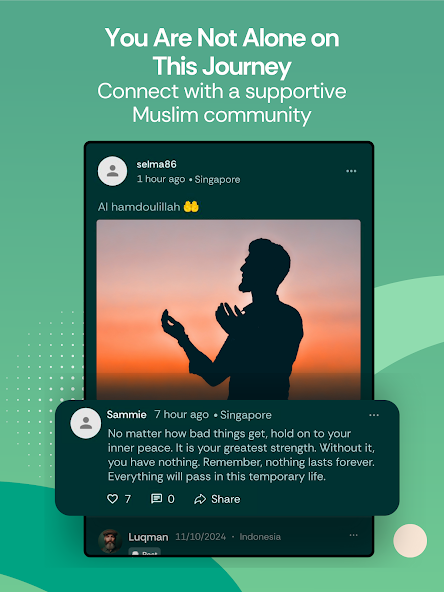
\includegraphics[width=0.6\textwidth]{muslimpro.png}
		\caption{Plateforme Muslim Pro}
		\label{fig:muslimpro}
	\end{figure}
	
	\textbf{Avantages}
	\begin{itemize}
		\item Large base d'utilisateurs mondiale offrant une forte visibilité communautaire.
		\item Fonctionnalités religieuses complètes : horaires de prière, Coran, Qibla.
	\end{itemize}
	
	\textbf{Inconvénients}
	\begin{itemize}
		\item L'application reste avant tout un outil de pratique individuelle, sans 
		véritable espace social dédié aux échanges et à la vie communautaire.
		\item Aucune fonctionnalité de formation, de masterclasses ou de gestion 
		d'événements n'est proposée.
		\item L'application n'est pas spécifiquement conçue pour les femmes musulmanes 
		et ne tient pas compte de leurs besoins particuliers.
	\end{itemize}
	
	\subsection{Salam Planet}
	
	Salam Planet se présente comme un réseau social destiné à la communauté musulmane 
	mondiale. Il permet le partage de publications, la discussion en groupe et la 
	consommation de contenus islamiques. La figure \ref{fig:salamplanet} présente 
	l'interface de Salam Planet.
	
	\begin{figure}[H]
		\centering
		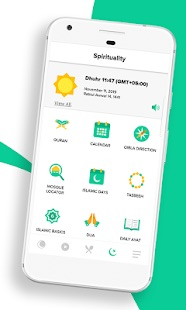
\includegraphics[width=0.6\textwidth]{salamplanet.png}
		\caption{Plateforme Salam Planet}
		\label{fig:salamplanet}
	\end{figure}
	
	\textbf{Avantages}
	\begin{itemize}
		\item Propose un espace social communautaire dédié aux musulmans avec 
		modération adaptée aux valeurs islamiques.
		\item Permet le partage de contenus, de publications et d'interactions 
		entre membres de la communauté.
	\end{itemize}
	
	\textbf{Inconvénients}
	\begin{itemize}
		\item La plateforme s'adresse à l'ensemble de la communauté musulmane sans 
		cibler spécifiquement les femmes ni leurs besoins propres.
		\item Absence de fonctionnalités éducatives telles que des masterclasses 
		ou des formations en ligne.
		\item Aucun système intégré de gestion et de participation à des événements 
		communautaires n'est disponible.
	\end{itemize}
	
	\subsection{Bilan et Positionnement de Soeurise}
	
	\begin{table}[H]
		\centering
		\renewcommand{\arraystretch}{1.4}
		\begin{tabular}{|l|c|c|c|}
			\hline
			\textbf{Fonctionnalité} & \textbf{Muslim Pro} & \textbf{Salam Planet} & \textbf{Soeurise} \\
			\hline
			Flux social communautaire & \textcolor{red}{\texttimes} & \textcolor{green}{\checkmark} & \textcolor{green}{\checkmark} \\
			\hline
			Dédié aux femmes musulmanes & \textcolor{red}{\texttimes} & \textcolor{red}{\texttimes} & \textcolor{green}{\checkmark} \\
			\hline
			Masterclasses et formations & \textcolor{red}{\texttimes} & \textcolor{red}{\texttimes} & \textcolor{green}{\checkmark} \\
			\hline
			Gestion d'événements & \textcolor{red}{\texttimes} & \textcolor{red}{\texttimes} & \textcolor{green}{\checkmark} \\
			\hline
			Espace privé et sécurisé & \textcolor{red}{\texttimes} & \textcolor{red}{\texttimes} & \textcolor{green}{\checkmark} \\
			\hline
		\end{tabular}
		\caption{Tableau comparatif des solutions existantes}
		\label{tab:comparatif}
	\end{table}
	
	\medskip
	
	Ce bilan confirme qu'aucune des solutions existantes ne répond pleinement aux besoins 
	des femmes musulmanes. \textbf{Soeurise} se distingue ainsi comme la première plateforme 
	à combiner, dans un seul et même espace, réseau social, formations, événements et 
	confidentialité, le tout pensé exclusivement pour elles.
	\section{Solution Proposée}
	
	En tenant compte des lacunes identifiées lors de l'étude des plateformes existantes, 
	nous avons conçu \textbf{Soeurise}, une solution complète qui répond concrètement 
	aux besoins des femmes musulmanes en quête d'un espace numérique sécurisé, inclusif 
	et adapté à leurs valeurs.
	
	En effet, le projet que nous avons réalisé est une plateforme mobile et web connectée 
	à une base de données robuste, offrant à ses utilisatrices un écosystème numérique 
	unifié autour de cinq fonctionnalités principales :
	
	\begin{itemize}
		\item \textbf{Un flux social :} permettre aux utilisatrices de publier, partager 
		leurs expériences et interagir avec leur communauté dans un environnement modéré 
		et bienveillant.
		
		\item \textbf{Des communautés de discussion :} offrir des espaces de groupe privés 
		et sécurisés, où les membres peuvent échanger librement autour de sujets qui leur 
		tiennent à cœur.
		
		\item \textbf{Des masterclasses et formations en ligne :} donner accès à des 
		contenus éducatifs de qualité, directement intégrés à la plateforme, pour apprendre 
		et évoluer sans quitter l'application.
		
		\item \textbf{Un système de gestion d'événements :} permettre à chaque utilisatrice 
		de découvrir, créer et participer à des événements communautaires, qu'ils soient 
		en ligne ou en présentiel.
		
		\item \textbf{Un profil utilisateur personnalisé :} offrir à chacune un espace 
		personnel regroupant son historique d'activité, ses événements et ses préférences, 
		pour une expérience vraiment sur mesure.
	\end{itemize}
	
	\medskip
	
	Grâce à cette approche globale et intégrée, \textbf{Soeurise} se positionne comme 
	la première plateforme à réunir en un seul endroit tout ce dont les femmes musulmanes 
	ont besoin pour s'exprimer, se former, se connecter et s'épanouir numériquement.
	
	\section{Méthodologies de Gestion de Projet}
	
	Avant de choisir la méthodologie qui allait guider notre travail, nous avons pris le 
	temps d'étudier les approches les plus répandues dans le domaine du génie logiciel. 
	Chacune présente des caractéristiques propres, et le bon choix dépend étroitement 
	du contexte, de la taille de l'équipe et de la nature du projet.
	
	\subsection{Cycle en V}
	
	Le Cycle en V est une méthode séquentielle classique, héritée des pratiques 
	industrielles. Elle structure le projet en phases successives et bien définies : 
	des spécifications jusqu'aux tests, chaque étape de développement est associée 
	à une phase de validation correspondante, formant ainsi un "V". Cette approche 
	offre une forte traçabilité et une documentation rigoureuse, ce qui la rend adaptée 
	aux projets aux exigences stables et bien connues dès le départ.
	
	\begin{itemize}
		\item[\textcolor{green}{\textbf{+}}] Documentation rigoureuse et traçabilité 
		complète à chaque étape du projet.
		\item[\textcolor{green}{\textbf{+}}] Structure claire et facile à comprendre, 
		idéale pour les projets aux exigences bien définies dès le départ.
		\item[\textcolor{green}{\textbf{+}}] Facilite la validation et la vérification 
		grâce à la correspondance entre phases de développement et phases de test.
		\item[\textcolor{red}{\textbf{--}}] Très faible flexibilité : toute modification 
		en cours de développement est coûteuse et difficile à intégrer.
		\item[\textcolor{red}{\textbf{--}}] Le produit final n'est livré qu'à la toute 
		fin du projet, ce qui retarde la détection des erreurs.
		\item[\textcolor{red}{\textbf{--}}] Ne convient pas aux projets dont les besoins 
		sont susceptibles d'évoluer au fil du temps.
	\end{itemize}
	
	\subsection{SCRUM}
	
	SCRUM est un cadre de travail agile basé sur des cycles de développement courts 
	et itératifs appelés \textit{sprints}, d'une durée généralement de deux semaines. 
	À la fin de chaque sprint, une version fonctionnelle et testée du produit est livrée, 
	permettant d'obtenir des retours rapides et d'ajuster le cap si nécessaire. SCRUM 
	repose sur trois piliers fondamentaux : la \textbf{transparence}, l'\textbf{inspection} 
	et l'\textbf{adaptation}.
	
	\begin{itemize}
		\item[\textcolor{green}{\textbf{+}}] Grande flexibilité : les besoins peuvent 
		évoluer et être intégrés facilement d'un sprint à l'autre.
		\item[\textcolor{green}{\textbf{+}}] Livraisons régulières et fonctionnelles 
		qui permettent de détecter les erreurs tôt et d'obtenir des retours continus.
		\item[\textcolor{green}{\textbf{+}}] Favorise la communication et la collaboration 
		au sein de l'équipe grâce aux rituels réguliers (daily, revue, rétrospective).
		\item[\textcolor{green}{\textbf{+}}] Particulièrement adapté aux équipes 
		distribuées et aux contextes de travail à distance ou international.
		\item[\textcolor{red}{\textbf{--}}] Nécessite une implication constante de toutes 
		les parties prenantes tout au long du projet.
		\item[\textcolor{red}{\textbf{--}}] La documentation peut être moins exhaustive 
		qu'avec des méthodes classiques, ce qui peut poser problème sur le long terme.
	\end{itemize}
	
	\subsection{Two Track Unified Process (2TUP)}
	
	Le 2TUP est une variante du Processus Unifié (UP) qui propose une approche originale 
	en séparant le projet en deux branches parallèles : une \textbf{branche fonctionnelle}, 
	centrée sur les besoins métier et les cas d'utilisation, et une \textbf{branche 
		technique}, dédiée à l'architecture et aux contraintes technologiques. Ces deux 
	branches convergent ensuite lors d'une phase de réalisation unifiée.
	
	\begin{itemize}
		\item[\textcolor{green}{\textbf{+}}] Séparation claire entre les aspects 
		fonctionnels et techniques, ce qui facilite le travail en parallèle.
		\item[\textcolor{green}{\textbf{+}}] Bien adaptée aux projets complexes 
		nécessitant une architecture technique solide et réfléchie.
		\item[\textcolor{green}{\textbf{+}}] Bonne traçabilité grâce à l'utilisation 
		intensive des diagrammes UML tout au long du processus.
		\item[\textcolor{red}{\textbf{--}}] Méthode relativement lourde et complexe 
		à mettre en œuvre, surtout pour une petite équipe.
		\item[\textcolor{red}{\textbf{--}}] Courbe d'apprentissage élevée et nécessite 
		une bonne maîtrise du Processus Unifié et d'UML.
		\item[\textcolor{red}{\textbf{--}}] Moins adaptée aux projets de taille réduite 
		ou aux délais courts comme un projet de fin d'études.
	\end{itemize}
	\section{Choix de la Méthodologie Adéquate}
	
	En récapitulant les points forts et les limites de chaque approche étudiée, il apparaît 
	clairement que notre projet nécessite une méthodologie à la fois flexible, itérative 
	et orientée vers des livraisons régulières. \textbf{Soeurise} est une plateforme 
	riche et évolutive, composée de cinq fonctionnalités majeures qui se développent 
	en parallèle, dans un contexte professionnel international où la communication et 
	l'adaptation rapide sont essentielles. Pour toutes ces raisons, nous avons retenu 
	la méthode \textbf{SCRUM}, car elle répond parfaitement aux exigences de notre projet 
	et au rythme de travail imposé par \textbf{Cafee Agency}.
	
	\begin{center}
		\(\Rightarrow\) \textit{Nous mettons en œuvre le cadre SCRUM pour la suite de notre travail.}
	\end{center}
	
	\section{Mise en Pratique du Processus SCRUM}
	
	SCRUM est un cadre de travail agile dont le principe central repose sur le découpage 
	du projet en cycles courts et itératifs appelés \textit{sprints}. Chaque sprint, 
	d'une durée de deux semaines, produit une version fonctionnelle et testable du produit, 
	permettant d'intégrer les retours au fur et à mesure et de garantir un avancement 
	continu et maîtrisé. Le processus SCRUM repose sur quatre caractéristiques 
	fondamentales :
	
	\begin{itemize}
		\item \textbf{Itératif et incrémental :} Le projet est découpé en sprints courts 
		et successifs. À chaque itération, une version enrichie et fonctionnelle de 
		la plateforme est produite, permettant de suivre précisément l'avancement global 
		du système.
		
		\item \textbf{Piloté par les priorités :} Les fonctionnalités sont classées par 
		ordre de priorité dans un \textit{Product Backlog}. Les éléments les plus critiques 
		sont traités en premier, ce qui réduit les risques d'échec et garantit que 
		l'essentiel est toujours livré.
		
		\item \textbf{Centré sur la collaboration :} SCRUM favorise une communication 
		constante entre les membres de l'équipe grâce à des rituels réguliers — réunions 
		quotidiennes, revues de sprint et rétrospectives — essentiels dans notre contexte 
		de travail à distance entre le New Mexico et l'Île-de-France.
		
		\item \textbf{Conduit par les besoins utilisateurs :} Chaque sprint est orienté 
		vers la livraison de valeur réelle pour les utilisatrices de \textbf{Soeurise}, 
		en gardant leurs besoins au centre de chaque décision de développement.
	\end{itemize}
	
	\medskip
	
	Comme l'illustre la figure \ref{fig:scrum}, le processus SCRUM adopté pour 
	\textbf{Soeurise} s'articule autour de trois éléments principaux :
	
	\begin{figure}[H]
		\centering
		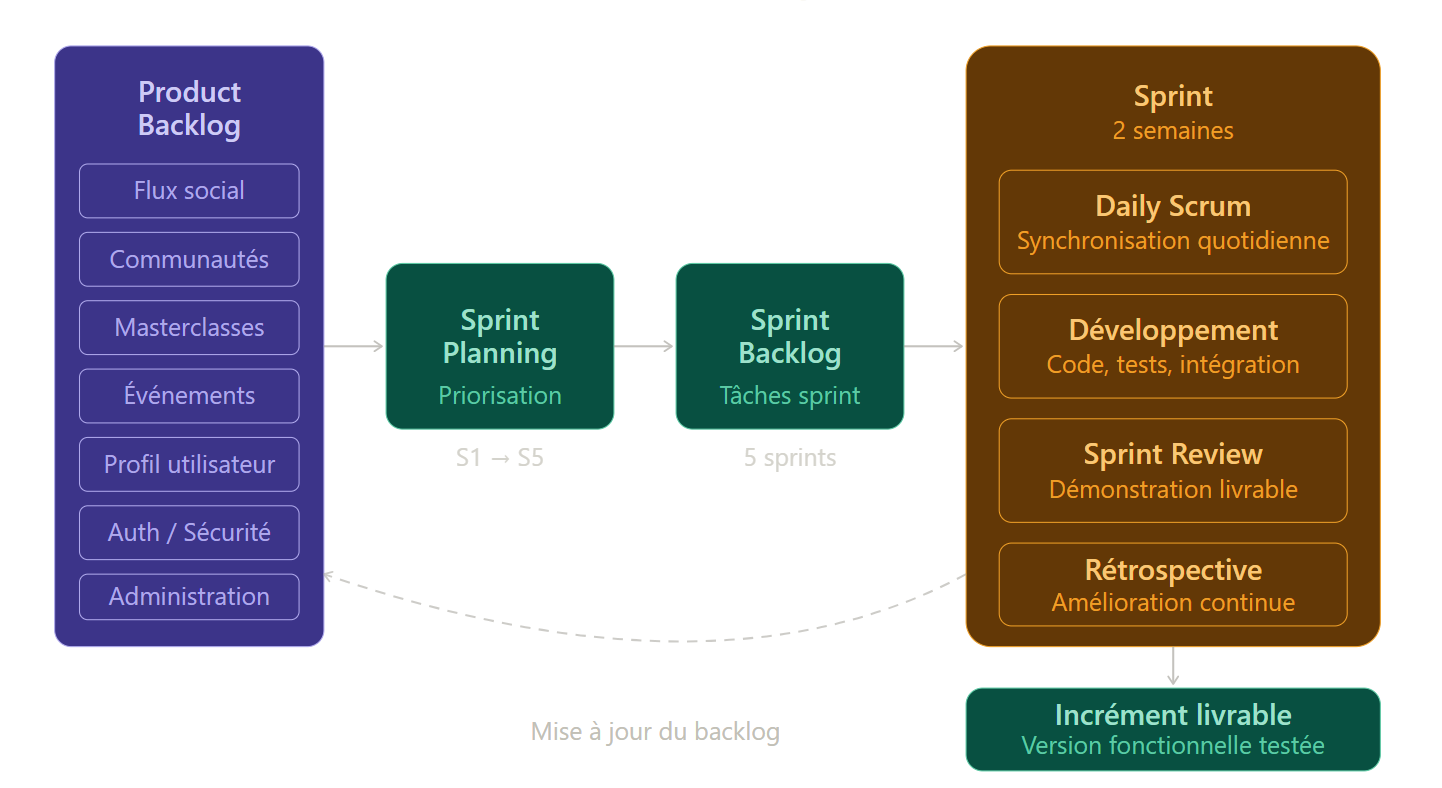
\includegraphics[width=0.75\textwidth]{scrum.png}
		\caption{Processus SCRUM -- Projet Soeurise}
		\label{fig:scrum}
	\end{figure}
	
	\subsection{Product Backlog}
	
	Le Product Backlog constitue la liste complète et priorisée de toutes les 
	fonctionnalités attendues de la plateforme \textbf{Soeurise}. Il regroupe l'ensemble 
	des besoins identifiés lors de la phase d'analyse : flux social, communautés, 
	masterclasses, événements et gestion du profil utilisateur. Ce backlog évolue tout 
	au long du projet en fonction des retours et des ajustements.
	
	\subsection{Sprint Planning \& Sprint Backlog}
	
	Au début de chaque sprint, une réunion de planification permet de sélectionner les 
	éléments prioritaires du Product Backlog à réaliser durant les deux semaines à venir. 
	Ces éléments forment le \textit{Sprint Backlog}, c'est-à-dire la liste des tâches 
	concrètes à accomplir durant le sprint en cours.
	
	\subsection{Livraison et Révision}
	
	À la fin de chaque sprint, une version fonctionnelle et testée de la plateforme est 
	livrée. Une revue de sprint permet d'évaluer ce qui a été accompli, d'identifier 
	les points d'amélioration et d'ajuster le backlog pour le sprint suivant, garantissant 
	ainsi une amélioration continue tout au long du développement.
	
	\section{Diagramme de Gantt}
	
	Le diagramme de Gantt est l'un des outils les plus utilisés en gestion de projet 
	pour représenter visuellement la planification et l'avancement des différentes tâches. 
	La colonne de gauche liste l'ensemble des sprints du projet, tandis que l'axe 
	horizontal représente la durée totale du développement, organisée en semaines.
	
	Le projet \textbf{Soeurise} a été planifié sur \textbf{dix semaines}, découpées 
	en cinq sprints de deux semaines chacun, allant de la mise en place de l'infrastructure 
	jusqu'à la finalisation et la livraison de la solution complète.
	
	La figure \ref{fig:gantt} présente le diagramme de Gantt de notre projet :
	
	\begin{figure}[H]
		\centering
		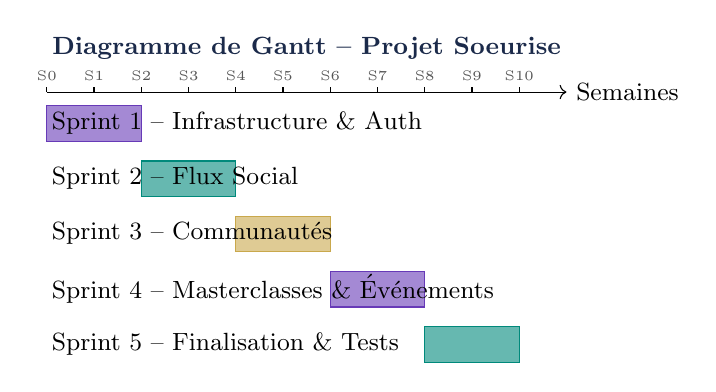
\begin{tikzpicture}[xscale=0.6,yscale=0.7]
			\node[font=\small\bfseries\color{cafeeNavy}]at(5.5,5.8)
			{Diagramme de Gantt -- Projet Soeurise};
			\draw[->](0,5)--(11,5)node[right,font=\small]{Semaines};
			\foreach \x in{0,1,...,10}{
				\draw(\x,5)--(\x,5.1);
				\node[font=\tiny,color=darkGray]at(\x,5.3){S\x};
			}
			\foreach \y/\lb/\st/\dur/\col in{
				4/Sprint 1 -- Infrastructure \& Auth/0/2/primaryPurple,
				3/Sprint 2 -- Flux Social/2/2/accentTeal,
				2/Sprint 3 -- Communautés/4/2/cafeeGold,
				1/Sprint 4 -- Masterclasses \& Événements/6/2/primaryPurple,
				0/Sprint 5 -- Finalisation \& Tests/8/2/accentTeal}
			{
				\fill[\col!60](\st,\y+0.1)rectangle(\st+\dur,\y+0.75);
				\draw[\col](\st,\y+0.1)rectangle(\st+\dur,\y+0.75);
				\node[font=\small,anchor=west]at(-0.1,\y+0.43){\lb};
			}
		\end{tikzpicture}
		\caption{Diagramme de Gantt -- Planification des sprints SCRUM}
		\label{fig:gantt}
	\end{figure}\section*{Conclusion}
	
	Au terme de ce premier chapitre, nous avons présenté le cadre général du projet 
	\textbf{Soeurise}, en décrivant notre organisme d'accueil \textbf{Cafee Agency}, 
	la problématique identifiée, l'étude des solutions existantes, ainsi que la 
	méthodologie \textbf{SCRUM} adoptée pour structurer notre développement. Le chapitre 
	suivant sera consacré à l'analyse et à la spécification des besoins de la plateforme.
	%% =========================================================
	%%  CHAPITRE 2
	%% =========================================================
	\chapter{Analyse et Spécification des Besoins}
	
	\section{Introduction}
	
	Avant de concevoir et de développer une solution logicielle, il est indispensable 
	de bien comprendre les besoins des utilisateurs et de définir avec précision ce que 
	le système doit accomplir. Ce chapitre constitue donc une étape fondamentale dans 
	notre démarche : il nous permet de poser les bases fonctionnelles et techniques de 
	la plateforme \textbf{Soeurise}, en identifiant les acteurs concernés, en capturant 
	les besoins fonctionnels à travers les cas d'utilisation, et en précisant les 
	contraintes non fonctionnelles que le système devra respecter.
	
	\section{Branche Fonctionnelle}
	
	\subsection{Identification des Acteurs}
	
	Un acteur représente toute entité externe qui interagit avec le système. Dans le 
	cadre de la plateforme \textbf{Soeurise}, trois acteurs principaux ont été identifiés :
	
	\begin{itemize}
		\item \textbf{L'utilisatrice (membre) :} C'est l'acteur central de la plateforme. 
		Elle s'inscrit, se connecte et accède à l'ensemble des fonctionnalités proposées : 
		publier dans le flux social, rejoindre des communautés, suivre des masterclasses, 
		participer à des événements et gérer son profil personnel.
		
		\item \textbf{L'administrateur :} Il assure la gestion et la modération de la 
		plateforme. Il dispose de droits étendus lui permettant de gérer les utilisatrices, 
		de modérer les contenus publiés, de superviser les communautés et de veiller 
		au bon fonctionnement général du système.
		
		\item \textbf{L'invitée (visiteur non connecté) :} Il s'agit de toute personne 
		accédant à la plateforme sans être authentifiée. Elle peut consulter certaines 
		informations publiques, mais ses interactions restent limitées jusqu'à ce qu'elle 
		crée un compte.
	\end{itemize}
	
	\subsection{Capture des Besoins Fonctionnels}
	
	Les besoins fonctionnels décrivent l'ensemble des actions et services que la 
	plateforme \textbf{Soeurise} doit offrir à ses utilisatrices. Ces besoins ont été 
	organisés par module fonctionnel :
	
	\subsubsection*{Module Authentification}
	\begin{itemize}
		\item Permettre à une nouvelle utilisatrice de créer un compte avec ses 
		informations personnelles.
		\item Permettre à une utilisatrice enregistrée de se connecter via son 
		adresse e-mail et son mot de passe.
		\item Permettre à une utilisatrice de réinitialiser son mot de passe 
		en cas d'oubli.
		\item Assurer la déconnexion sécurisée de la session en cours.
	\end{itemize}
	
	\subsubsection*{Module Flux Social}
	\begin{itemize}
		\item Permettre à une utilisatrice de créer, modifier et supprimer 
		ses publications.
		\item Afficher un fil d'actualité personnalisé regroupant les publications 
		des membres et des communautés suivies.
		\item Permettre d'interagir avec les publications via des réactions 
		et des commentaires.
	\end{itemize}
	
	\subsubsection*{Module Communautés}
	\begin{itemize}
		\item Permettre à une utilisatrice de créer une communauté, de la 
		paramétrer et d'en gérer les membres.
		\item Permettre de rejoindre une communauté existante et d'y participer 
		via la messagerie de groupe.
		\item Permettre à l'administrateur de modérer les communautés et 
		leurs contenus.
	\end{itemize}
	
	\subsubsection*{Module Masterclasses}
	\begin{itemize}
		\item Permettre aux utilisatrices de consulter le catalogue des 
		masterclasses et formations disponibles.
		\item Permettre l'accès au contenu des formations (vidéos, documents) 
		directement depuis l'application.
		\item Permettre à l'administrateur d'ajouter, modifier ou supprimer 
		des masterclasses.
	\end{itemize}
	
	\subsubsection*{Module Événements}
	\begin{itemize}
		\item Permettre la création et la publication d'événements en ligne 
		ou en présentiel.
		\item Permettre aux utilisatrices de s'inscrire à un événement et 
		de consulter leur calendrier personnel.
		\item Permettre à l'administrateur de gérer l'ensemble des événements 
		de la plateforme.
	\end{itemize}
	
	\subsubsection*{Module Profil Utilisateur}
	\begin{itemize}
		\item Permettre à chaque utilisatrice de consulter et de modifier 
		ses informations personnelles et sa photo de profil.
		\item Afficher l'historique des activités, des événements auxquels 
		elle a participé et des formations suivies.
		\item Permettre la personnalisation des préférences de l'application.
	\end{itemize}
	
	\subsection{Capture des Besoins Non Fonctionnels}
	
	Au-delà des fonctionnalités, une application de qualité doit également répondre 
	à un ensemble de contraintes non fonctionnelles qui garantissent sa fiabilité, 
	ses performances et son accessibilité. Pour \textbf{Soeurise}, ces contraintes 
	sont les suivantes :
	
	\begin{itemize}
		\item \textbf{Sécurité :} La plateforme doit garantir la confidentialité 
		des données personnelles de ses utilisatrices. L'authentification repose 
		sur des tokens \textbf{JWT}, les mots de passe sont hachés via 
		\textbf{bcryptjs}, et l'API est protégée contre les attaques courantes 
		grâce à \textbf{Helmet} et \textbf{Express-Rate-Limit}.
		
		\item \textbf{Performance :} L'application doit offrir des temps de 
		réponse rapides et une navigation fluide, même lors de pics d'utilisation. 
		La base de données \textbf{MongoDB} a été choisie pour sa flexibilité 
		et ses capacités de montée en charge.
		
		\item \textbf{Disponibilité :} La plateforme doit être accessible en 
		permanence, avec un taux de disponibilité élevé, pour garantir une 
		expérience utilisateur continue et fiable.
		
		\item \textbf{Compatibilité multiplateforme :} Grâce au framework 
		\textbf{Flutter}, l'application est déployable sur Android, iOS, Web 
		et Windows, offrant ainsi une expérience cohérente quel que soit 
		l'appareil utilisé.
		
		\item \textbf{Ergonomie et accessibilité :} L'interface doit être 
		intuitive, agréable et accessible à toutes les utilisatrices, 
		indépendamment de leur niveau de familiarité avec les outils numériques. 
		Le design suit les principes du \textbf{Material Design 3} en mode sombre.
		
		\item \textbf{Maintenabilité :} Le code source doit être bien structuré, 
		documenté et facilement maintenable. La documentation interactive de 
		l'API est assurée par \textbf{Swagger}, facilitant les évolutions 
		futures de la plateforme.
	\end{itemize}
	\section{Diagramme de cas d'utilisation general}
	\begin{figure}[H]
		\centering
		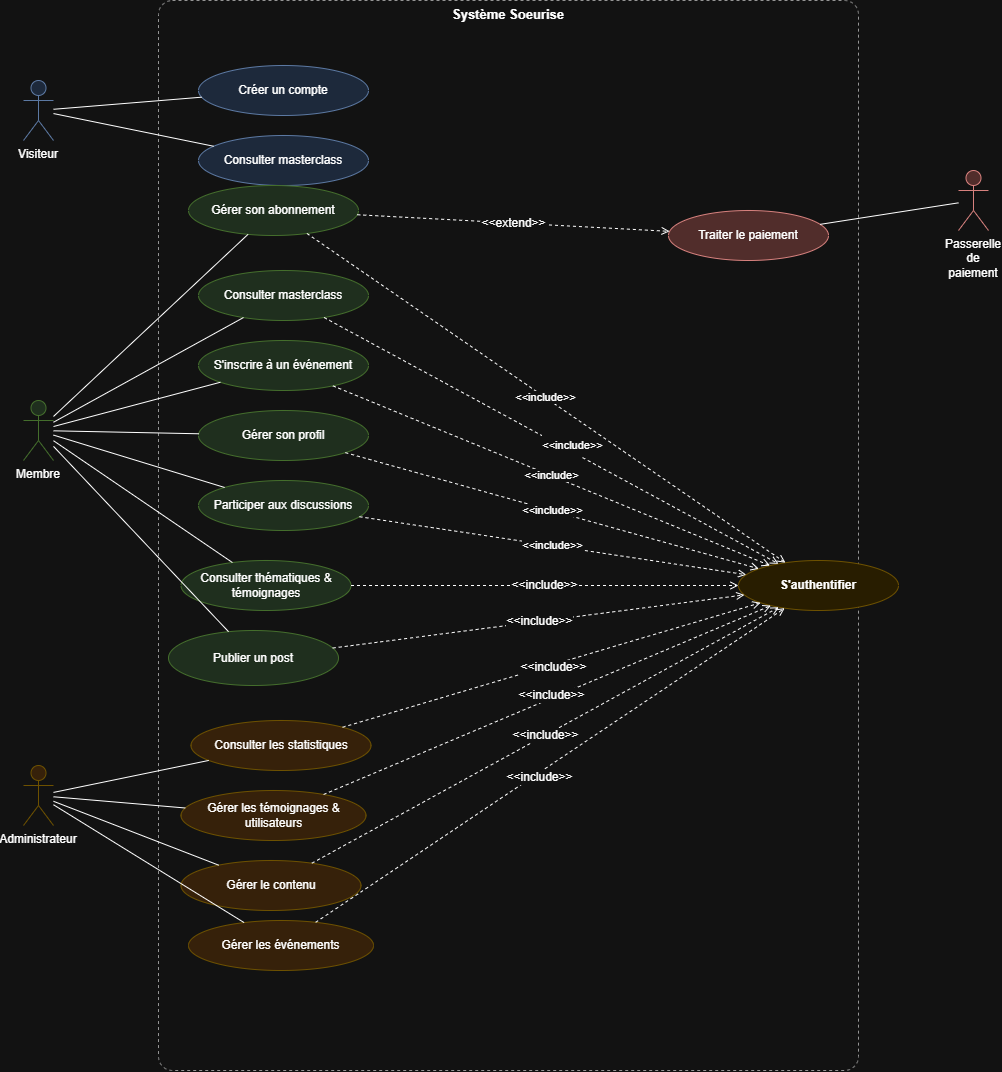
\includegraphics[width=1\textwidth]{diagramme de cas d'utilisation.drawio (1).png}
		\caption{diagramme de cas d'utilisation général }
		\label{fig:}
	\end{figure}
	
	\section{Raffinement des cas d'utilisation <<gérer contenu>>}
	\begin{figure}[H]
		\centering
		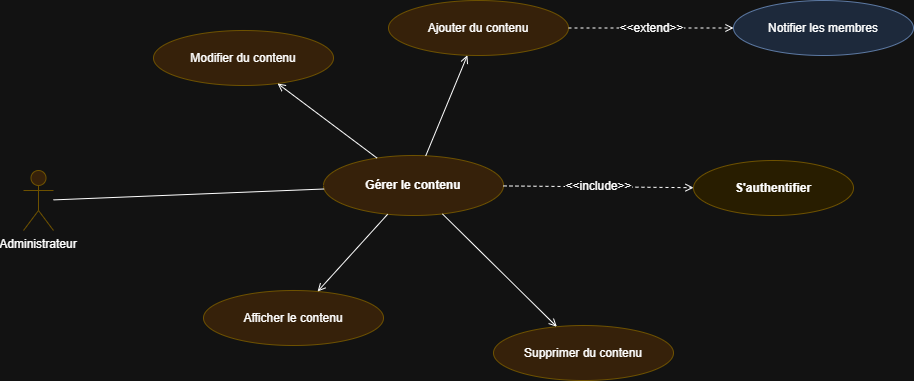
\includegraphics[width=1\textwidth]{raffinement gerer contenu.drawio.png}
		\caption{diagramme de cas d'utilisation <<gérer contenu>> }
		\label{fig:}
	\end{figure}
	Le tableau \ref{tab:uc-gerer-contenu} décrit le cas d'utilisation détaillé 
	« Ajouter du contenu ».
	
	\begin{table}[H]
		\centering
		\renewcommand{\arraystretch}{1.4}
		\begin{tabular}{|p{3.5cm}|p{9.5cm}|}
			\hline
			\multicolumn{2}{|c|}{\textbf{Sommaire d'identification}} \\
			\hline
			Cas d'utilisation & Ajouter du contenu \\
			\hline
			Acteur & Administrateur \\
			\hline
			Résumé & Action permettant à l'administrateur d'ajouter un nouveau contenu sur la plateforme Soeurise (masterclass, événement ou publication). \\
			\hline
			\multicolumn{2}{|c|}{\textbf{Description des enchaînements}} \\
			\hline
			Pré-conditions & L'administrateur doit être authentifié sur la plateforme. \\
			\hline
			Post-conditions & Le contenu est ajouté et devient visible pour les utilisatrices de la plateforme. \\
			\hline
			\multicolumn{2}{|c|}{\textbf{Scénario nominal}} \\
			\hline
			\multicolumn{2}{|p{13cm}|}{%
				1 - L'administrateur clique sur « Gérer le contenu » dans le menu de l'interface d'administration.\newline
				2 - Le système affiche la liste des contenus existants.\newline
				3 - L'administrateur clique sur le bouton « Ajouter un contenu ».\newline
				4 - Le système affiche un formulaire de saisie.\newline
				5 - L'administrateur remplit tous les champs requis (titre, description, type, fichiers associés).\newline
				6 - L'administrateur clique sur le bouton « Enregistrer ».\newline
				7 - Le système valide les données et enregistre le nouveau contenu.\newline
				8 - Le système affiche un message de confirmation et met à jour la liste des contenus.%
			} \\
			\hline
			\multicolumn{2}{|c|}{\textbf{Scénario d'exception}} \\
			\hline
			\multicolumn{2}{|p{13cm}|}{%
				E1 : Erreur de connexion — le système affiche un message d'erreur et invite l'administrateur à se reconnecter.\newline
				E2 : Champs obligatoires manquants — le système signale les champs incomplets et bloque l'enregistrement.\newline
				E3 : Format de fichier invalide — le système rejette le fichier et affiche un message indiquant les formats acceptés.%
			} \\
			\hline
		\end{tabular}
		\caption{Description détaillée du cas d'utilisation «Ajouter du contenu»}
		\label{tab:uc-gerer-contenu}
	\end{table}
	\section{Raffinement des cas d'utilisation <<s'inscrire à un événement >>}
	\begin{figure}[H]
		\centering
		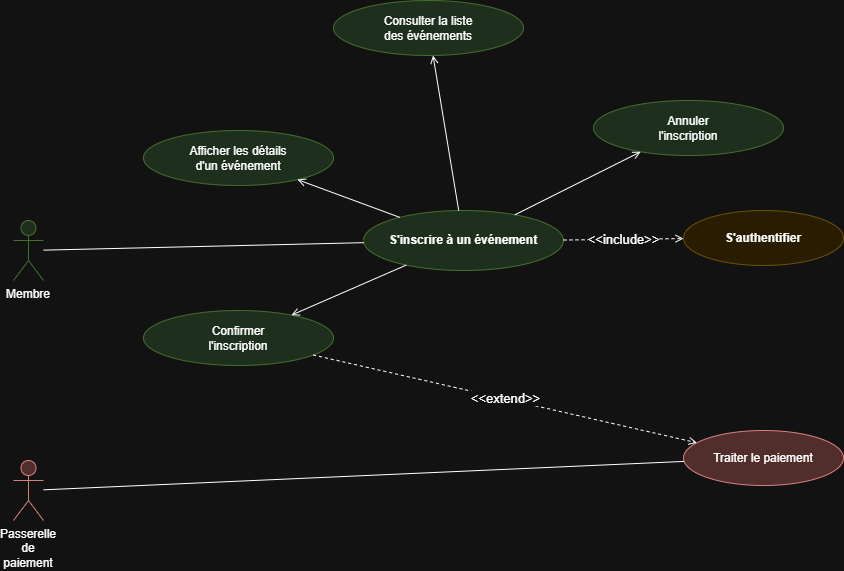
\includegraphics[width=1\textwidth]{raffinement event.drawio.png}
		\caption{diagramme de cas d'utilisation <<s'inscrire à un événement>> }
		\label{fig:}
	\end{figure}
	Le tableau \ref{tab:uc-inscrire-evenement} décrit le cas d'utilisation détaillé 
	« S'inscrire à un événement ».
	
	\begin{table}[H]
		\centering
		\renewcommand{\arraystretch}{1.4}
		\begin{tabular}{|p{3.5cm}|p{9.5cm}|}
			\hline
			\multicolumn{2}{|c|}{\textbf{Sommaire d'identification}} \\
			\hline
			Cas d'utilisation & S'inscrire à un événement \\
			\hline
			Acteur & Membre \\
			\hline
			Résumé & Action permettant à un membre authentifié de consulter les événements disponibles et de s'inscrire à un événement de son choix, en ligne ou en présentiel. \\
			\hline
			\multicolumn{2}{|c|}{\textbf{Description des enchaînements}} \\
			\hline
			Pré-conditions & Le membre doit être authentifié sur la plateforme. \\
			\hline
			Post-conditions & Le membre est inscrit à l'événement et reçoit une confirmation d'inscription. \\
			\hline
			\multicolumn{2}{|c|}{\textbf{Scénario nominal}} \\
			\hline
			\multicolumn{2}{|p{13cm}|}{%
				1 - Le membre clique sur « Événements » dans le menu de navigation.\newline
				2 - Le système affiche la liste des événements disponibles.\newline
				3 - Le membre sélectionne un événement pour consulter ses détails.\newline
				4 - Le système affiche les informations complètes de l'événement (date, lieu, description).\newline
				5 - Le membre clique sur le bouton « S'inscrire ».\newline
				6 - Si l'événement est payant, le système redirige vers la passerelle de paiement.\newline
				7 - Le membre confirme son inscription.\newline
				8 - Le système enregistre l'inscription et envoie une confirmation au membre.%
			} \\
			\hline
			\multicolumn{2}{|c|}{\textbf{Scénario d'exception}} \\
			\hline
			\multicolumn{2}{|p{13cm}|}{%
				E1 : Erreur de connexion — le système affiche un message d'erreur et invite le membre à se reconnecter.\newline
				E2 : Places épuisées — le système informe le membre que l'événement est complet et lui propose d'autres événements disponibles.\newline
				E3 : Échec du paiement — le système annule l'inscription et invite le membre à réessayer avec un autre moyen de paiement.%
			} \\
			\hline
		\end{tabular}
		\caption{Description détaillée du cas d'utilisation «S'inscrire à un événement»}
		\label{tab:uc-inscrire-evenement}
	\end{table}
	\section{Raffinement des cas d'utilisation <<publier un post>>}
	\begin{figure}[H]
		\centering
		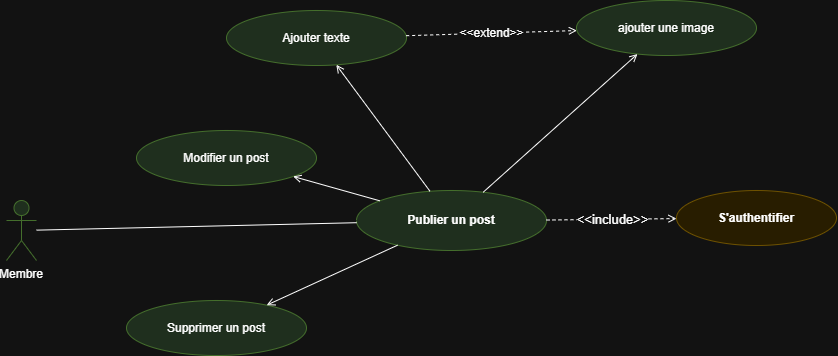
\includegraphics[width=1\textwidth]{raffinement pub post.drawio.png}
		\caption{diagramme de cas d'utilisation <<publier un post >> }
		\label{fig:}
	\end{figure}
	Le tableau \ref{tab:uc-publier-post} décrit le cas d'utilisation détaillé 
	« Publier un post ».
	
	\begin{table}[H]
		\centering
		\renewcommand{\arraystretch}{1.4}
		\begin{tabular}{|p{3.5cm}|p{9.5cm}|}
			\hline
			\multicolumn{2}{|c|}{\textbf{Sommaire d'identification}} \\
			\hline
			Cas d'utilisation & Publier un post \\
			\hline
			Acteur & Membre \\
			\hline
			Résumé & Action permettant à un membre authentifié de créer et publier un post dans le flux social de la plateforme Soeurise, avec la possibilité d'ajouter du texte, une image, de modifier ou de supprimer ses publications. \\
			\hline
			\multicolumn{2}{|c|}{\textbf{Description des enchaînements}} \\
			\hline
			Pré-conditions & Le membre doit être authentifié sur la plateforme. \\
			\hline
			Post-conditions & Le post est publié et devient visible pour les autres membres de la communauté. \\
			\hline
			\multicolumn{2}{|c|}{\textbf{Scénario nominal}} \\
			\hline
			\multicolumn{2}{|p{13cm}|}{%
				1 - Le membre accède au flux social depuis le menu de navigation.\newline
				2 - Le système affiche le fil d'actualité avec les publications existantes.\newline
				3 - Le membre clique sur le bouton « Créer un post ».\newline
				4 - Le système affiche un éditeur de publication.\newline
				5 - Le membre rédige son texte et ajoute éventuellement une image.\newline
				6 - Le membre clique sur le bouton « Publier ».\newline
				7 - Le système valide le contenu et publie le post.\newline
				8 - Le système affiche le nouveau post en tête du flux social.%
			} \\
			\hline
			\multicolumn{2}{|c|}{\textbf{Scénario d'exception}} \\
			\hline
			\multicolumn{2}{|p{13cm}|}{%
				E1 : Erreur de connexion — le système affiche un message d'erreur et invite le membre à se reconnecter.\newline
				E2 : Contenu vide — le système signale que le post ne peut pas être publié sans texte et bloque la publication.\newline
				E3 : Format d'image invalide — le système rejette le fichier image et affiche un message indiquant les formats acceptés.%
			} \\
			\hline
		\end{tabular}
		\caption{Description détaillée du cas d'utilisation «Publier un post»}
		\label{tab:uc-publier-post}
	\end{table}
	\section{Branche Technique}
	
	La réussite d'un projet logiciel repose en grande partie sur la pertinence des 
	choix technologiques effectués en amont. Pour développer \textbf{Soeurise}, nous 
	avons sélectionné des technologies modernes, éprouvées et parfaitement adaptées 
	aux exigences d'une application communautaire cross-platform. Cette section présente 
	l'ensemble des langages, frameworks et outils qui ont constitué notre environnement 
	de développement.
	
	\subsection{Flutter \& Dart — Frontend}
	
	\textbf{Flutter} est un framework open-source développé par Google, permettant de 
	créer des applications natives pour Android, iOS, Web et Desktop à partir d'une 
	seule base de code. C'est la technologie principale choisie pour développer 
	l'interface utilisateur de \textbf{Soeurise}. Son langage associé, \textbf{Dart}, 
	est un langage orienté objet, fortement typé et optimisé pour la performance des 
	interfaces graphiques.
	
	Flutter s'est imposé comme un choix naturel pour notre projet pour plusieurs raisons :
	\begin{itemize}
		\item Un seul code source déployable sur Android, iOS, Web et Windows.
		\item Des performances natives grâce au moteur de rendu graphique Skia.
		\item Un système de widgets riche et personnalisable, conforme au 
		\textbf{Material Design 3}.
		\item Un thème sombre (\textit{Dark Mode}) avec un fond \texttt{\#121212} 
		et une couleur d'accentuation Deep Purple \texttt{\#673AB7}.
	\end{itemize}
	
	Les principaux packages Flutter utilisés dans le projet sont :
	\begin{itemize}
		\item \textbf{http} : pour communiquer avec l'API backend via des requêtes REST.
		\item \textbf{shared\_preferences} : pour stocker localement le token JWT 
		et maintenir la session utilisateur.
		\item \textbf{image\_picker} : pour permettre à l'utilisatrice d'ajouter 
		des images (photo de profil, publications).
		\item \textbf{google\_fonts} : pour une typographie personnalisée et moderne.
		\item \textbf{url\_launcher} et \textbf{webview\_flutter} : pour ouvrir 
		des liens externes et intégrer des vues web (vidéos de masterclasses, 
		liens d'événements).
	\end{itemize}
	
	\subsection{Node.js \& Express.js — Backend}
	
	\textbf{Node.js} est un environnement d'exécution JavaScript côté serveur, 
	reconnu pour sa légèreté, sa rapidité et sa capacité à gérer un grand nombre 
	de connexions simultanées. Il constitue le cœur du backend de \textbf{Soeurise}. 
	Associé au framework \textbf{Express.js}, il nous a permis de concevoir une 
	API RESTful robuste, claire et facilement maintenable, qui gère l'ensemble de 
	la logique métier de l'application.
	
	\subsection{MongoDB \& Mongoose — Base de données}
	
	\textbf{MongoDB} est une base de données NoSQL orientée documents, reconnue 
	pour sa flexibilité et ses capacités de montée en charge. Elle stocke les données 
	sous format JSON, ce qui la rend particulièrement adaptée à une application 
	communautaire avec des structures de données variées et évolutives comme 
	les publications, les profils utilisateurs ou les événements.
	
	\textbf{Mongoose} est l'ODM (\textit{Object Data Modeling}) utilisé pour 
	interfacer Node.js avec MongoDB. Il permet de définir des schémas de données 
	structurés et d'interagir avec la base de données de manière simple et sécurisée.
	
	\subsection{Sécurité}
	
	La sécurité étant au cœur des valeurs de \textbf{Soeurise}, plusieurs mécanismes 
	ont été mis en place pour protéger les données des utilisatrices :
	
	\begin{itemize}
		\item \textbf{JSON Web Token (JWT)} : génération de tokens d'accès sécurisés 
		pour authentifier les utilisatrices sans stocker de session côté serveur.
		\item \textbf{bcryptjs} : hachage sécurisé des mots de passe avant leur 
		stockage en base de données.
		\item \textbf{Helmet} : protection de l'API contre les attaques XSS et 
		autres vulnérabilités HTTP courantes.
		\item \textbf{Express-Rate-Limit} : limitation du nombre de requêtes par 
		adresse IP pour prévenir les attaques par force brute.
		\item \textbf{Joi} : validation rigoureuse des données envoyées par 
		l'application avant tout traitement côté serveur.
	\end{itemize}
	
	\subsection{Gestion des fichiers et Documentation}
	
	\begin{itemize}
		\item \textbf{Multer} : middleware utilisé pour intercepter et sauvegarder 
		les fichiers envoyés par les utilisatrices (images de profil, publications).
		\item \textbf{Swagger} : génération automatique d'une documentation 
		interactive de l'API grâce aux packages \texttt{swagger-ui-express} et 
		\texttt{swagger-jsdoc}, facilitant la maintenance et les évolutions futures 
		de la plateforme.
	\end{itemize}
	
	\section{Conclusion}
	Ce chapitre a été consacré à la description des besoins fonctionnels et techniques.
	Dans le prochain chapitre, nous abordons les étapes de conception et l’architecture
	technique, qui sont cruciales pour concevoir la solution du projet.
	%% =========================================================
	%%  CHAPITRE 3
	%% =========================================================
	\chapter{Étude Conceptuelle}
	
	\section{Introduction}
	
	Après avoir analysé les besoins fonctionnels et techniques de la plateforme 
	\textbf{Soeurise}, il est désormais temps de passer à l'étape de conception. 
	Ce chapitre constitue le pont entre l'analyse des besoins et la phase de 
	réalisation : il s'agit de traduire ce que le système doit faire en une 
	représentation structurée et rigoureuse de comment il va le faire.
	
	Pour ce faire, nous nous appuyons sur le langage de modélisation \textbf{UML}, 
	qui nous permettra de représenter visuellement l'architecture, le comportement 
	et les interactions au sein de notre système. Nous présenterons ensuite 
	l'architecture logique retenue, avant de détailler les diagrammes de classes 
	et de séquence qui modélisent concrètement le fonctionnement de la plateforme.
	
	\section{Présentation du Langage UML}
	
	\textbf{UML} (\textit{Unified Modeling Language}) est un langage de modélisation 
	graphique standardisé, largement adopté dans le domaine du génie logiciel. 
	Il permet de visualiser, spécifier, construire et documenter les artefacts 
	d'un système logiciel de manière claire et universellement compréhensible.
	
	Comme l'illustre la figure \ref{fig:uml-axes}, UML organise la modélisation 
	d'un système autour de trois axes complémentaires :
	
	\begin{itemize}
		\item \textbf{L'axe Fonctionnel} — ce que le système FAIT : représenté 
		par le diagramme de cas d'utilisation et le diagramme d'activités.
		
		\item \textbf{L'axe Statique} — ce que le système EST : représenté 
		par le diagramme de classes, le diagramme d'objets, le diagramme 
		de composants et le diagramme de déploiement.
		
		\item \textbf{L'axe Dynamique} — comment le système ÉVOLUE : représenté 
		par le diagramme de séquence, le diagramme de collaboration et le 
		diagramme d'états-transitions.
	\end{itemize}
	
	\begin{figure}[H]
		\centering
		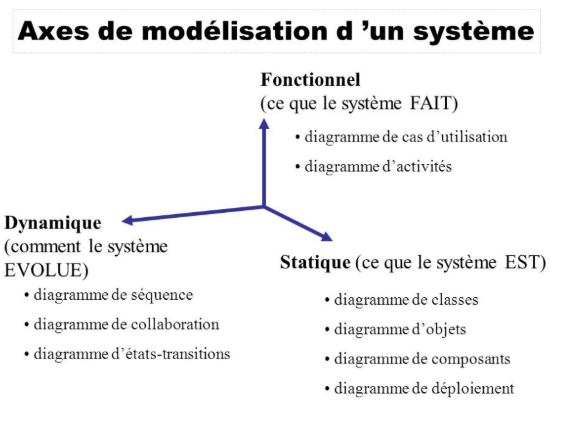
\includegraphics[width=0.75\textwidth]{uml_axes.png}
		\caption{Axes de modélisation d'un système UML}
		\label{fig:uml-axes}
	\end{figure}
	
	Dans le cadre de ce projet, nous avons utilisé :
	\begin{itemize}
		\item Le \textbf{diagramme de cas d'utilisation} (axe fonctionnel) — 
		présenté au chapitre précédent.
		\item Le \textbf{diagramme de classes} (axe statique) — pour modéliser 
		la structure des données de \textbf{Soeurise}.
		\item Les \textbf{diagrammes de séquence} (axe dynamique) — pour 
		illustrer les interactions entre les composants du système.
	\end{itemize}
	
	\section{Architecture Logique}
	
	\subsection{Présentation de l'Architecture 3-Tiers}
	
	L'architecture retenue pour la plateforme \textbf{Soeurise} est une architecture 
	\textbf{3-tiers} (trois couches), également appelée architecture client-serveur 
	multicouche. Ce modèle architectural organise le système en trois niveaux 
	distincts et indépendants, chacun ayant un rôle bien défini :
	
	\begin{itemize}
		\item \textbf{La couche Présentation (Frontend) :} c'est l'interface avec 
		laquelle l'utilisatrice interagit directement. Dans notre cas, elle est 
		développée avec \textbf{Flutter}, ce qui permet de déployer l'application 
		sur Android, iOS, Web et Windows à partir d'une seule base de code. 
		Cette couche est responsable de l'affichage des données et de la collecte 
		des actions de l'utilisatrice, qu'elle transmet ensuite au serveur via 
		des requêtes HTTP.
		
		\item \textbf{La couche Métier (Backend) :} c'est le cerveau du système. 
		Développée avec \textbf{Node.js} et \textbf{Express.js}, elle abrite 
		toute la logique applicative : traitement des requêtes, vérification des 
		droits d'accès, application des règles métier et communication avec la 
		base de données. Elle expose une \textbf{API RESTful} sécurisée que le 
		frontend consomme pour récupérer ou envoyer des données.
		
		\item \textbf{La couche Données (Base de données) :} c'est là que résident 
		toutes les données de la plateforme. Nous avons opté pour \textbf{MongoDB}, 
		une base de données NoSQL orientée documents, interfacée via \textbf{Mongoose}. 
		Cette couche est totalement isolée du frontend et n'est accessible qu'à 
		travers le backend, ce qui garantit la sécurité et l'intégrité des données.
	\end{itemize}
	
	\subsection{Avantages de cette Architecture}
	
	Le choix de l'architecture 3-tiers pour \textbf{Soeurise} n'est pas anodin. 
	Ce modèle présente plusieurs avantages concrets qui correspondent parfaitement 
	aux besoins et aux contraintes de notre projet :
	
	\begin{itemize}
		\item \textbf{Séparation des responsabilités :} chaque couche est 
		indépendante et n'a qu'un seul rôle bien défini. Cela rend le code 
		plus lisible, plus facile à maintenir et à faire évoluer dans le temps.
		
		\item \textbf{Sécurité renforcée :} la base de données n'est jamais 
		exposée directement au frontend. Toutes les requêtes passent obligatoirement 
		par le backend, qui applique les contrôles de sécurité nécessaires 
		(authentification JWT, validation des données, protection contre les attaques).
		
		\item \textbf{Scalabilité :} chaque couche peut être mise à l'échelle 
		indépendamment en fonction des besoins. Si le nombre d'utilisatrices 
		augmente considérablement, il est possible de renforcer uniquement 
		le backend ou la base de données sans toucher au reste du système.
		
		\item \textbf{Portabilité :} grâce à \textbf{Flutter}, la couche 
		présentation est déployable sur plusieurs plateformes sans modifier 
		l'architecture globale, ce qui offre une grande flexibilité pour 
		les évolutions futures de \textbf{Soeurise}.
		
		\item \textbf{Maintenabilité :} la séparation claire entre les couches 
		facilite le travail en équipe, chaque développeur pouvant intervenir 
		sur une couche sans impacter les autres.
	\end{itemize}
	\section{Diagramme de Classes}
	
	Le diagramme de classes permet de visualiser de manière globale la plateforme 
	\textbf{Soeurise}, en décrivant les relations et les interactions entre ses 
	différentes entités. Chacune des classes possède ses propres attributs et méthodes, 
	et collabore avec les autres pour assurer le bon fonctionnement de l'ensemble 
	du système. Dans la figure \ref{fig:class-diagram}, nous observons le diagramme 
	de classes de notre application, montrant toutes les classes impliquées, leurs 
	relations et les associations entre elles. Il est formé principalement par 
	\textbf{dix classes} et chaque classe possède des attributs et
	des méthodes.chacune jouant un rôle précis et complémentaire au sein 
	de l'architecture de \textbf{Soeurise} :
	\begin{figure}[H]
		\centering
		
\includegraphics[width=1\textwidth]{diagramme de classeee.drawio.png}
		\caption{Diagramme de classes — Plateforme Soeurise}
		\label{fig:class-diagram}
	\end{figure}
	\subsection{Diagramme de séquence « S'authentifier »}
	
	La figure \ref{fig:login-diagram} présente le diagramme de séquence 
	« S'authentifier » et illustre les interactions entre les différents 
	composants du système lors du processus de connexion.
	
	Pour s'authentifier, l'utilisatrice accède à la page de connexion et 
	saisit ses identifiants — son adresse email et son mot de passe — dans 
	l'interface de connexion. Cette interface transmet ensuite les identifiants 
	au contrôleur, qui se charge de les valider en consultant la base de données. 
	La base de données retourne le résultat de la vérification au contrôleur, 
	qui traite la réponse selon deux scénarios possibles : si les identifiants 
	sont corrects, la session est ouverte et l'utilisatrice est redirigée vers 
	l'écran d'accueil ; dans le cas contraire, elle reste sur la page de 
	connexion et un message d'erreur lui est affiché.
	
	\begin{figure}[H]
		\centering
		\includegraphics[width=0.95\textwidth]{login diagram.drawio.png}
		\caption{Diagramme de séquence «S'authentifier»}
		\label{fig:login-diagram}
	\end{figure}
	\newpage
	\subsection{Diagramme de séquence « S'inscrire à un événement »}
	
	La figure \ref{fig:event-diagram} présente le diagramme de séquence 
	« S'inscrire à un événement » et illustre les interactions entre les 
	différents composants du système lors du processus d'inscription.
	
	Pour s'inscrire à un événement, l'utilisatrice accède à la liste des 
	événements disponibles depuis l'interface dédiée. Cette interface 
	transmet la demande au contrôleur, qui interroge la base de données 
	pour récupérer les événements disponibles et les afficher à l'utilisatrice. 
	Une fois l'événement de son choix sélectionné, elle clique sur 
	« S'inscrire ». Le système distingue alors deux scénarios : si 
	l'événement est gratuit, l'inscription est directement enregistrée 
	en base de données et une confirmation est affichée à l'utilisatrice ; 
	si l'événement est payant, le système redirige vers le contrôleur de 
	paiement pour traiter la transaction, et ce n'est qu'après confirmation 
	du paiement que l'inscription est validée et la confirmation affichée.
	
	\begin{figure}[H]
		\centering
		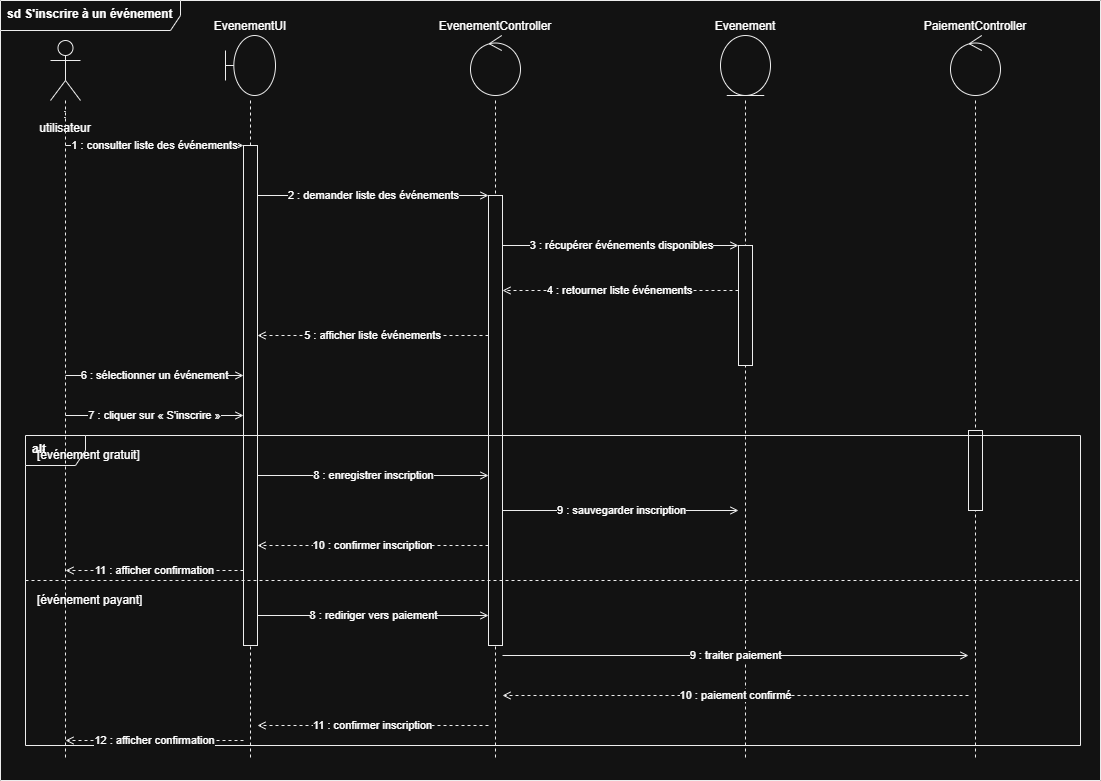
\includegraphics[width=0.95\textwidth]{event_Diagram.drawio.png}
		\caption{Diagramme de séquence «S'inscrire à un événement»}
		\label{fig:event-diagram}
	\end{figure}
	\newpage
	\subsection{Diagramme de séquence « Gérer le contenu »}
	
	La figure \ref{fig:contenu-diagram} présente le diagramme de séquence 
	« Gérer le contenu » et illustre les interactions entre l'administrateur 
	et les différents composants du système lors des opérations de gestion 
	du contenu de la plateforme.
	
	Pour gérer le contenu, l'administrateur accède à l'interface dédiée, 
	qui transmet la demande au contrôleur afin de récupérer et d'afficher 
	la liste des contenus existants. À partir de cet écran, trois actions 
	sont possibles : si l'administrateur souhaite \textbf{ajouter} un nouveau 
	contenu, il remplit le formulaire et le soumet — le contrôleur sauvegarde 
	alors le nouveau contenu en base de données et confirme l'ajout ; s'il 
	souhaite \textbf{modifier} un contenu existant, il sélectionne l'élément 
	concerné, apporte ses modifications et les envoie au contrôleur, qui met 
	à jour la base de données et confirme la modification ; enfin, s'il 
	souhaite \textbf{supprimer} un contenu, il sélectionne l'élément et 
	confirme la suppression — le contrôleur procède alors à la suppression 
	en base de données et affiche un message de confirmation à l'administrateur.
	
	\begin{figure}[H]
		\centering
		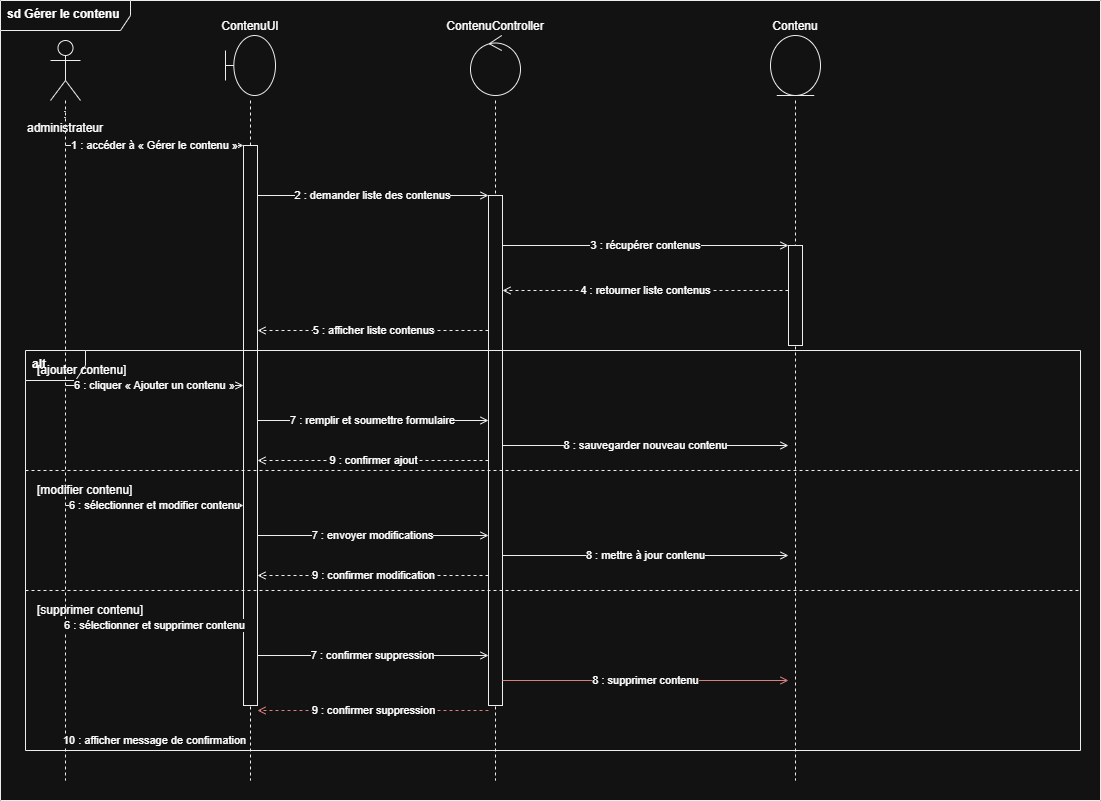
\includegraphics[width=0.95\textwidth]{contenu_diagram.drawio.png}
		\caption{Diagramme de séquence «Gérer le contenu»}
		\label{fig:contenu-diagram}
	\end{figure}
	\section*{Conclusion}
	
	Ce chapitre a débuté par une présentation du langage de modélisation 
	\textbf{UML} et de ses trois axes fondamentaux, suivie d'une description 
	de l'architecture \textbf{3-tiers} adoptée pour la plateforme 
	\textbf{Soeurise}. Nous avons ensuite exploré deux types de modélisations 
	complémentaires : la modélisation \textbf{statique}, représentée par le 
	diagramme de classes qui structure l'ensemble des entités du système, et 
	la modélisation \textbf{dynamique}, illustrée par trois diagrammes de 
	séquence décrivant les scénarios les plus importants de la plateforme — 
	l'authentification, l'inscription à un événement et la gestion du contenu. 
	Forts de cette conception solide et bien structurée, nous sommes désormais 
	prêts à aborder le dernier chapitre, dans lequel nous présenterons 
	concrètement la réalisation de notre projet à travers les interfaces 
	finales de la plateforme \textbf{Soeurise}.
	%% =========================================================
	%%  CHAPITRE 4
	%% =========================================================
	\chapter{Réalisation}
	
	\section{Introduction}
	
	Après avoir posé les bases conceptuelles et architecturales de la plateforme 
	\textbf{Soeurise} dans les chapitres précédents, nous abordons dans ce dernier 
	chapitre la phase de réalisation. Il s'agit de présenter concrètement le fruit 
	de notre travail, en décrivant l'environnement dans lequel l'application a été 
	développée, puis en illustrant les différentes interfaces qui composent la 
	plateforme. Ce chapitre constitue ainsi la vitrine de notre projet, où les 
	choix de conception se transforment en une solution numérique tangible et 
	fonctionnelle.
	
	\section{Environnement de Développement}
	
	Pour mener à bien le développement de \textbf{Soeurise}, nous avons eu 
	recours à un ensemble d'outils logiciels soigneusement choisis pour leur 
	efficacité, leur complémentarité et leur adéquation avec les technologies 
	utilisées dans le projet.
	
	\begin{itemize}
		\item \textbf{Visual Studio Code :} éditeur de code principal utilisé 
		pour le développement du backend Node.js/Express.js. Léger, extensible 
		et doté d'un écosystème de plugins riche, il a constitué notre 
		environnement de développement quotidien pour l'écriture et le débogage 
		du code serveur.
		
		\item \textbf{Android Studio :} environnement de développement intégré 
		utilisé pour le développement de l'application Flutter. Il offre un 
		émulateur Android intégré, un débogueur performant et une intégration 
		native avec le SDK Flutter et Dart.
		
		\item \textbf{Postman :} outil indispensable pour tester et valider 
		les endpoints de notre API RESTful. Il nous a permis de simuler des 
		requêtes HTTP (GET, POST, PUT, DELETE) et de vérifier les réponses 
		du serveur tout au long du développement.
		
		\item \textbf{MongoDB Compass :} interface graphique officielle de 
		MongoDB, utilisée pour visualiser, explorer et manipuler les données 
		stockées dans notre base de données directement depuis une interface 
		intuitive.
		
		\item \textbf{Git \& GitHub :} outils de gestion de versions utilisés 
		pour suivre l'évolution du code source, gérer les branches de 
		développement et sauvegarder le projet de manière sécurisée tout au 
		long du stage.
		
		\item \textbf{draw.io :} outil de modélisation utilisé pour concevoir 
		l'ensemble des diagrammes UML du projet (cas d'utilisation, classes, 
		séquences).
		
		\item \textbf{Swagger UI :} interface de documentation interactive 
		générée automatiquement pour notre API, permettant de consulter et 
		de tester les endpoints directement depuis le navigateur.
		
		\item \textbf{Overleaf :} éditeur \LaTeX{} collaboratif en ligne utilisé 
		pour la rédaction et la mise en forme du présent rapport de projet de 
		fin d'études. Il offre une compilation en temps réel, une gestion 
		simplifiée des packages et un environnement accessible depuis n'importe 
		quel navigateur, sans installation préalable.
	\end{itemize}
	\section{Présentation de l'Application}
	
	Dans cette section, nous présentons les différentes interfaces de la 
	plateforme \textbf{Soeurise}, telles qu'elles ont été développées et 
	livrées à l'issue du projet.
	
	\subsection{Interface d'Onboarding}
	
	Au premier lancement de l'application, l'utilisatrice est accueillie 
	par trois écrans d'introduction qui présentent les valeurs et les 
	fonctionnalités clés de \textbf{Soeurise}, avant de l'inviter à 
	rejoindre la communauté.
	
	\begin{figure}[H]
		\centering
		\begin{minipage}{0.32\textwidth}
			\centering
			
\includegraphics[width=\textwidth]{onboarding1.png}
			\caption{Onboarding — Bienvenue}
			\label{fig:onboarding1}
		\end{minipage}
		\hfill
		\begin{minipage}{0.32\textwidth}
			\centering
			
\includegraphics[width=\textwidth]{onboarding2.png}
			\caption{Onboarding — Apprenez}
			\label{fig:onboarding2}
		\end{minipage}
		\hfill
		\begin{minipage}{0.32\textwidth}
			\centering
			
\includegraphics[width=\textwidth]{onboarding3.png}
			\caption{Onboarding — Connectez-vous}
			\label{fig:onboarding3}
		\end{minipage}
	\end{figure}
	
	\subsection{Interface d'Authentification}
	
	L'interface d'authentification constitue le point d'entrée de la 
	plateforme \textbf{Soeurise}. Elle se compose de deux écrans : 
	l'écran de connexion et l'écran d'inscription.
	
	\begin{figure}[H]
		\centering
		\begin{minipage}{0.48\textwidth}
			\centering
			
\includegraphics[width=\textwidth]{screen_login.png}
			\caption{Écran de connexion}
			\label{fig:screen-login}
		\end{minipage}
		\hfill
		\begin{minipage}{0.48\textwidth}
			\centering
			
\includegraphics[width=\textwidth]{screen_register.png}
			\caption{Écran d'inscription}
			\label{fig:screen-register}
		\end{minipage}
	\end{figure}
	
	L'écran de connexion permet à une utilisatrice déjà inscrite de 
	s'authentifier via son email et son mot de passe. L'écran d'inscription 
	permet à une nouvelle venue de créer son compte en renseignant ses 
	informations personnelles — prénom, nom, nom d'utilisateur, email et 
	mot de passe — avant de rejoindre la communauté.
	
	\subsection{Interface du Flux Social}
	
	Le flux social constitue le cœur de l'expérience sur \textbf{Soeurise}. 
	Il affiche les publications des membres de la communauté et permet à 
	chaque utilisatrice d'interagir avec le contenu partagé.
	
	\begin{figure}[H]
		\centering
		
\includegraphics[width=0.85\textwidth]{screen_home.png}
		\caption{Écran d'accueil — fil d'actualité}
		\label{fig:screen-home}
	\end{figure}
	
	\begin{figure}[H]
		\centering
		
\includegraphics[width=0.85\textwidth]{screen_home2.png}
		\caption{Fil d'actualité — abonnements}
		\label{fig:screen-home2}
	\end{figure}
	
	\subsubsection*{Création d'un post}
	
	L'écran de création de post permet à une utilisatrice de rédiger une 
	nouvelle publication, d'y ajouter une photo ou un emoji, et de la 
	partager avec toute la communauté en un clic.
	
	\begin{figure}[H]
		\centering
		
\includegraphics[width=0.85\textwidth]{screen_create_post.png}
		\caption{Écran de création d'une publication}
		\label{fig:screen-create-post}
	\end{figure}
	
	\subsection{Interface des Communautés}
	
	L'écran des communautés affiche l'ensemble des espaces de discussion 
	disponibles sur la plateforme, organisés en vedette et en liste complète. 
	Chaque utilisatrice peut rejoindre librement une communauté selon ses 
	centres d'intérêt.
	
	\begin{figure}[H]
		\centering
		
\includegraphics[width=0.85\textwidth]{screen_communities.png}
		\caption{Écran liste des communautés}
		\label{fig:screen-communities}
	\end{figure}
	
	\subsection{Interface des Masterclasses}
	
	L'écran des masterclasses présente le catalogue complet des formations 
	disponibles sur \textbf{Soeurise}. Chaque formation est présentée avec 
	une image de couverture, un titre, une brève description et le nom de 
	la formatrice.
	
	\begin{figure}[H]
		\centering
		
\includegraphics[width=0.85\textwidth]{screen_masterclass.png}
		\caption{Écran liste des masterclasses}
		\label{fig:screen-masterclass}
	\end{figure}
	
	\subsection{Interface des Événements}
	
	L'écran des événements affiche l'ensemble des rencontres disponibles 
	sur la plateforme, qu'elles soient en présentiel ou en ligne. Chaque 
	événement est présenté avec sa date, son lieu et un bouton d'inscription 
	direct.
	
	\begin{figure}[H]
		\centering
		
\includegraphics[width=0.85\textwidth]{screen_events.png}
		\caption{Écran liste des événements}
		\label{fig:screen-events}
	\end{figure}
	
	\subsection{Interface du Profil Utilisateur}
	
	L'interface de profil offre à chaque utilisatrice un espace personnel 
	complet. Elle peut y consulter ses statistiques (publications, abonnés, 
	suivies), accéder à son historique d'activité (masterclasses suivies, 
	événements inscrits, communautés rejointes) et modifier ses informations 
	personnelles.
	
	\begin{figure}[H]
		\centering
		\begin{minipage}{0.48\textwidth}
			\centering
			
\includegraphics[width=\textwidth]{screen_profile.png}
			\caption{Écran profil utilisateur}
			\label{fig:screen-profile}
		\end{minipage}
		\hfill
		\begin{minipage}{0.48\textwidth}
			\centering
			
\includegraphics[width=\textwidth]{screen_profile2.png}
			\caption{Écran activité utilisateur}
			\label{fig:screen-profile2}
		\end{minipage}
	\end{figure}
	
	\begin{figure}[H]
		\centering
		
\includegraphics[width=0.85\textwidth]{screen_edit_profile.png}
		\caption{Modal de modification du profil}
		\label{fig:screen-edit-profile}
	\end{figure}
	
	\subsection{Interface des Paramètres}
	
	L'écran des paramètres permet à chaque utilisatrice de personnaliser 
	son expérience sur la plateforme. Il regroupe les préférences générales 
	(notifications, mode sombre, langue) ainsi que les options de 
	confidentialité (mot de passe, visibilité du profil, utilisateurs 
	bloqués) et les informations légales relatives à \textbf{Soeurise}.
	
	\begin{figure}[H]
		\centering
		
\includegraphics[width=0.85\textwidth]{screen_settings.png}
		\caption{Écran des paramètres}
		\label{fig:screen-settings}
	\end{figure}
	
	\subsection{Interface d'Administration}
	
	L'interface d'administration est réservée aux administrateurs de la 
	plateforme. Elle leur permet notamment de créer et gérer les événements 
	de la communauté via un formulaire dédié, accessible directement depuis 
	l'écran des événements.
	
	\begin{figure}[H]
		\centering
		
\includegraphics[width=0.85\textwidth]{screen_admin_event.png}
		\caption{Interface d'administration — Création d'un événement}
		\label{fig:screen-admin-event}
	\end{figure}
	
	\section*{Conclusion}
	
	Ce dernier chapitre nous a permis de présenter concrètement la 
	plateforme \textbf{Soeurise} dans son état final. Après avoir décrit 
	l'environnement logiciel utilisé tout au long du développement, nous 
	avons illustré les différentes interfaces de l'application, couvrant 
	l'ensemble des fonctionnalités développées : onboarding, authentification, 
	flux social, communautés, masterclasses, événements, profil utilisateur, 
	paramètres et administration. Ce travail représente l'aboutissement d'un 
	projet ambitieux, mené avec rigueur et passion, dans le but d'offrir aux 
	femmes musulmanes un espace numérique qui leur est entièrement dédié.
	\chapter*{Conclusion Générale}
	\addcontentsline{toc}{chapter}{Conclusion Générale}
	
	Au terme de ce projet de fin d'études, nous pouvons affirmer avec fierté 
	que l'aventure \textbf{Soeurise} a été bien plus qu'un simple exercice 
	académique. Elle a représenté pour nous une expérience humaine et technique 
	complète, qui nous a permis de mobiliser l'ensemble des compétences acquises 
	tout au long de notre formation en \textbf{Génie Logiciel et Systèmes 
		d'Information} à l'\textbf{Institut Supérieur d'Informatique et de Gestion 
		de Kairouan}.
	
	\medskip
	
	Tout a commencé par un constat simple mais profond : malgré l'omniprésence 
	des réseaux sociaux, les femmes musulmanes ne disposaient d'aucun espace 
	numérique véritablement pensé pour elles. Ni les grandes plateformes 
	généralistes, trop impersonnelles et inadaptées, ni les rares applications 
	religieuses existantes, trop limitées dans leurs fonctionnalités, ne 
	répondaient à ce besoin réel et criant. C'est de cette conviction qu'est 
	née l'idée de \textbf{Soeurise} : offrir enfin à cette communauté mondiale 
	un espace sécurisé, inclusif et chaleureux, où elles peuvent s'exprimer, 
	apprendre, se rencontrer et s'épanouir librement.
	
	\medskip
	
	Pour concrétiser cette vision, nous avons suivi une démarche rigoureuse 
	et structurée, organisée en quatre grandes étapes. Dans un premier temps, 
	nous avons établi le \textbf{cadre général du projet} au sein de 
	\textbf{Cafee Agency}, en définissant la problématique, en étudiant 
	les solutions existantes et en adoptant la méthodologie \textbf{SCRUM} 
	pour piloter notre développement de manière agile et efficace. Dans un 
	second temps, nous avons procédé à une \textbf{analyse approfondie des 
		besoins}, en identifiant les différents acteurs du système et en 
	spécifiant l'ensemble des fonctionnalités attendues à travers des cas 
	d'utilisation détaillés et des besoins non fonctionnels précis. La 
	troisième étape nous a conduits vers l'\textbf{étude conceptuelle}, 
	où nous avons modélisé notre système à l'aide des outils UML — diagramme 
	de classes, diagrammes de séquence — et défini l'architecture 3-tiers 
	qui structure la plateforme. Enfin, la phase de \textbf{réalisation} 
	nous a permis de donner vie à l'ensemble de ces réflexions, en 
	développant une application cross-platform fonctionnelle, aussi bien 
	sur le plan technique que visuel.
	
	\medskip
	
	Sur le plan technique, \textbf{Soeurise} repose sur des technologies 
	modernes et éprouvées : \textbf{Flutter} et \textbf{Dart} pour une 
	expérience utilisateur fluide et cohérente sur toutes les plateformes, 
	\textbf{Node.js} et \textbf{Express.js} pour un backend robuste et 
	performant, et \textbf{MongoDB} pour une base de données flexible et 
	scalable. La sécurité a été placée au cœur de nos choix techniques, 
	avec l'authentification par \textbf{JWT}, le hachage des mots de passe 
	via \textbf{bcryptjs} et la protection de l'API contre les attaques 
	courantes.
	
	\medskip
	
	La plateforme livrée à l'issue de ce projet intègre cinq grandes 
	fonctionnalités : un \textbf{flux social} pour partager et interagir, 
	des \textbf{communautés de discussion} pour se retrouver entre sœurs, 
	des \textbf{masterclasses} pour apprendre et évoluer, un \textbf{système 
		d'événements} pour se rencontrer en ligne ou en présentiel, et un 
	\textbf{profil personnalisé} pour chaque utilisatrice. L'ensemble est 
	accessible via une interface soignée, intuitive et bienveillante, pensée 
	pour mettre à l'aise dès le premier écran.
	
	\medskip
	
	Ce projet nous a également offert une expérience professionnelle précieuse 
	au sein d'une agence internationale, \textbf{Cafee Agency}, qui nous a 
	appris ce que signifie véritablement travailler en équipe sur un projet 
	ambitieux, avec des contraintes réelles de temps, de qualité et de 
	communication à distance. Nous en ressortons avec une vision plus mature 
	du métier de développeur, une meilleure maîtrise des outils et des 
	bonnes pratiques du secteur, et surtout, la satisfaction d'avoir contribué 
	à quelque chose qui a du sens.
	
	\medskip
	
	Bien sûr, ce projet n'est qu'un point de départ. De nombreuses 
	perspectives d'évolution restent envisageables pour les versions 
	futures de \textbf{Soeurise} : l'intégration d'un \textbf{système de 
		notifications en temps réel} via WebSockets, le développement d'un 
	\textbf{moteur de recommandation} personnalisé pour les masterclasses 
	et les événements, l'ajout d'une \textbf{messagerie privée} entre 
	membres, ou encore le déploiement de la plateforme sur les stores 
	officiels Android et iOS pour toucher le plus grand nombre.
	
	\medskip
	
	En définitive, \textbf{Soeurise} est bien plus qu'une application. 
	C'est un projet de cœur, né d'un besoin réel, construit avec passion 
	et livré avec fierté. Nous espérons sincèrement qu'il pourra, un jour, 
	apporter de la valeur à toutes ces femmes qui méritent un espace 
	numérique qui leur ressemble.
	
\end{document}